%==================== chapter3_27.tex ====================

\clearpage
\thispagestyle{plain}

\begingroup
\fontsize{16pt}{19.2pt}\selectfont
\justifying
\XeTeXlinebreakskip=0pt plus 1pt minus 0.5pt
\setlength{\parindent}{1.5cm}
\setlength{\parskip}{0pt}

\begin{sloppypar}
	\begin{enumerate}[start=4]  % เริ่มที่ 2 (ต่อจาก 1)
		\item \textbf{Web Application ผู้จัดการประกวด}
	\end{enumerate}
\end{sloppypar}

\begin{figure}[h]
	\centering
	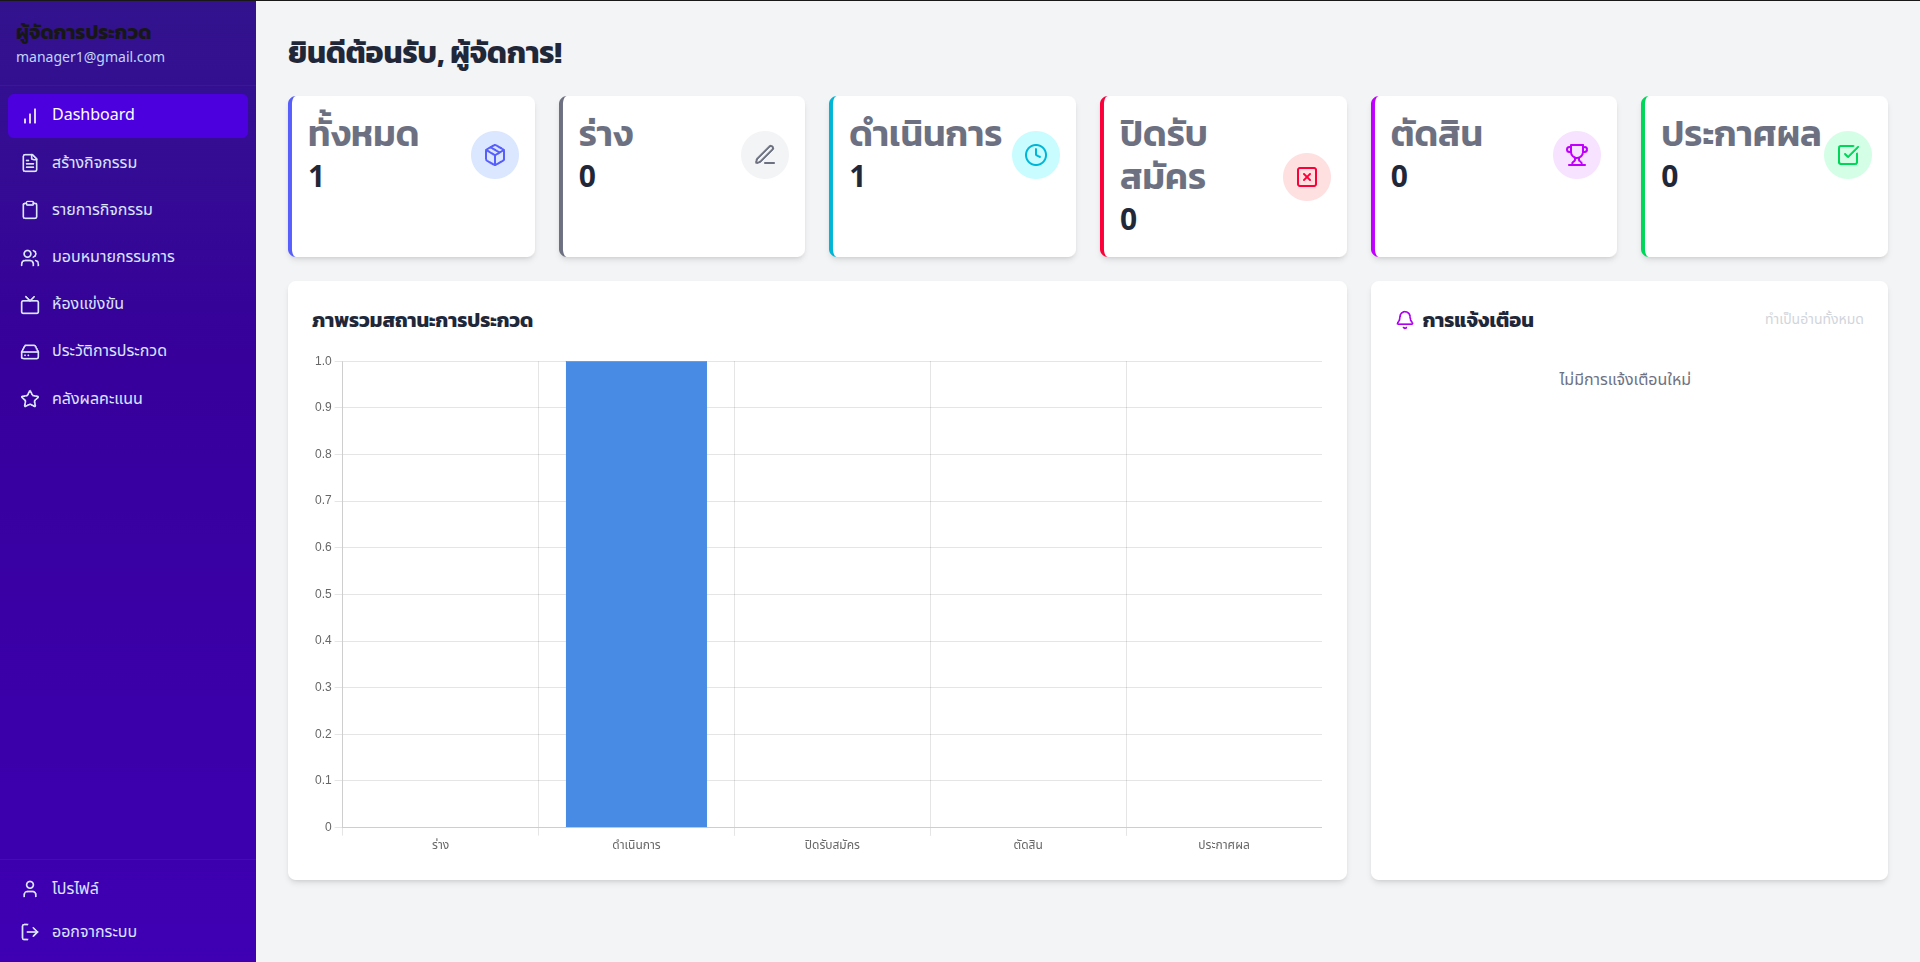
\includegraphics[width=0.8\linewidth]{MG1}
	\caption{หน้าหลักของผู้จัดการประกวด}
\end{figure}

\indent หน้านี้คือหน้า แดชบอร์ด (Dashboard) ผู้จัดการประกวด จัดการสามารถ ดูภาพรวม และ เข้าถึงเครื่องมือจัดการ ทั้งหมดได้ สรุปสถานะการประกวด: ตรงกลางหน้าจะมี การ์ดสรุปตัวเลข บอกชัดเจนว่าตอนนี้มีกิจกรรมทั้งหมดกี่รายการ, อยู่ในสถานะ "ร่าง", "กำลังดำเนินการ", หรือ "ประกาศผล" ไปแล้วกี่รายการ ซึ่งข้อมูลนี้จะถูกสรุปเป็น กราฟแท่ง ด้านล่างเพื่อให้เห็นภาพรวมได้ง่ายขึ้น ดูการแจ้งเตือน: ทางด้านขวาจะมีกล่อง "การแจ้งเตือน" คอยบอกข่าวสารสำคัญๆ เช่น มีผู้เชี่ยวชาญตอบรับคำเชิญ หรือมีกิจกรรมที่ใกล้จะเริ่มแล้ว

\vspace{\baselineskip}

\begin{figure}[h]
	\centering
	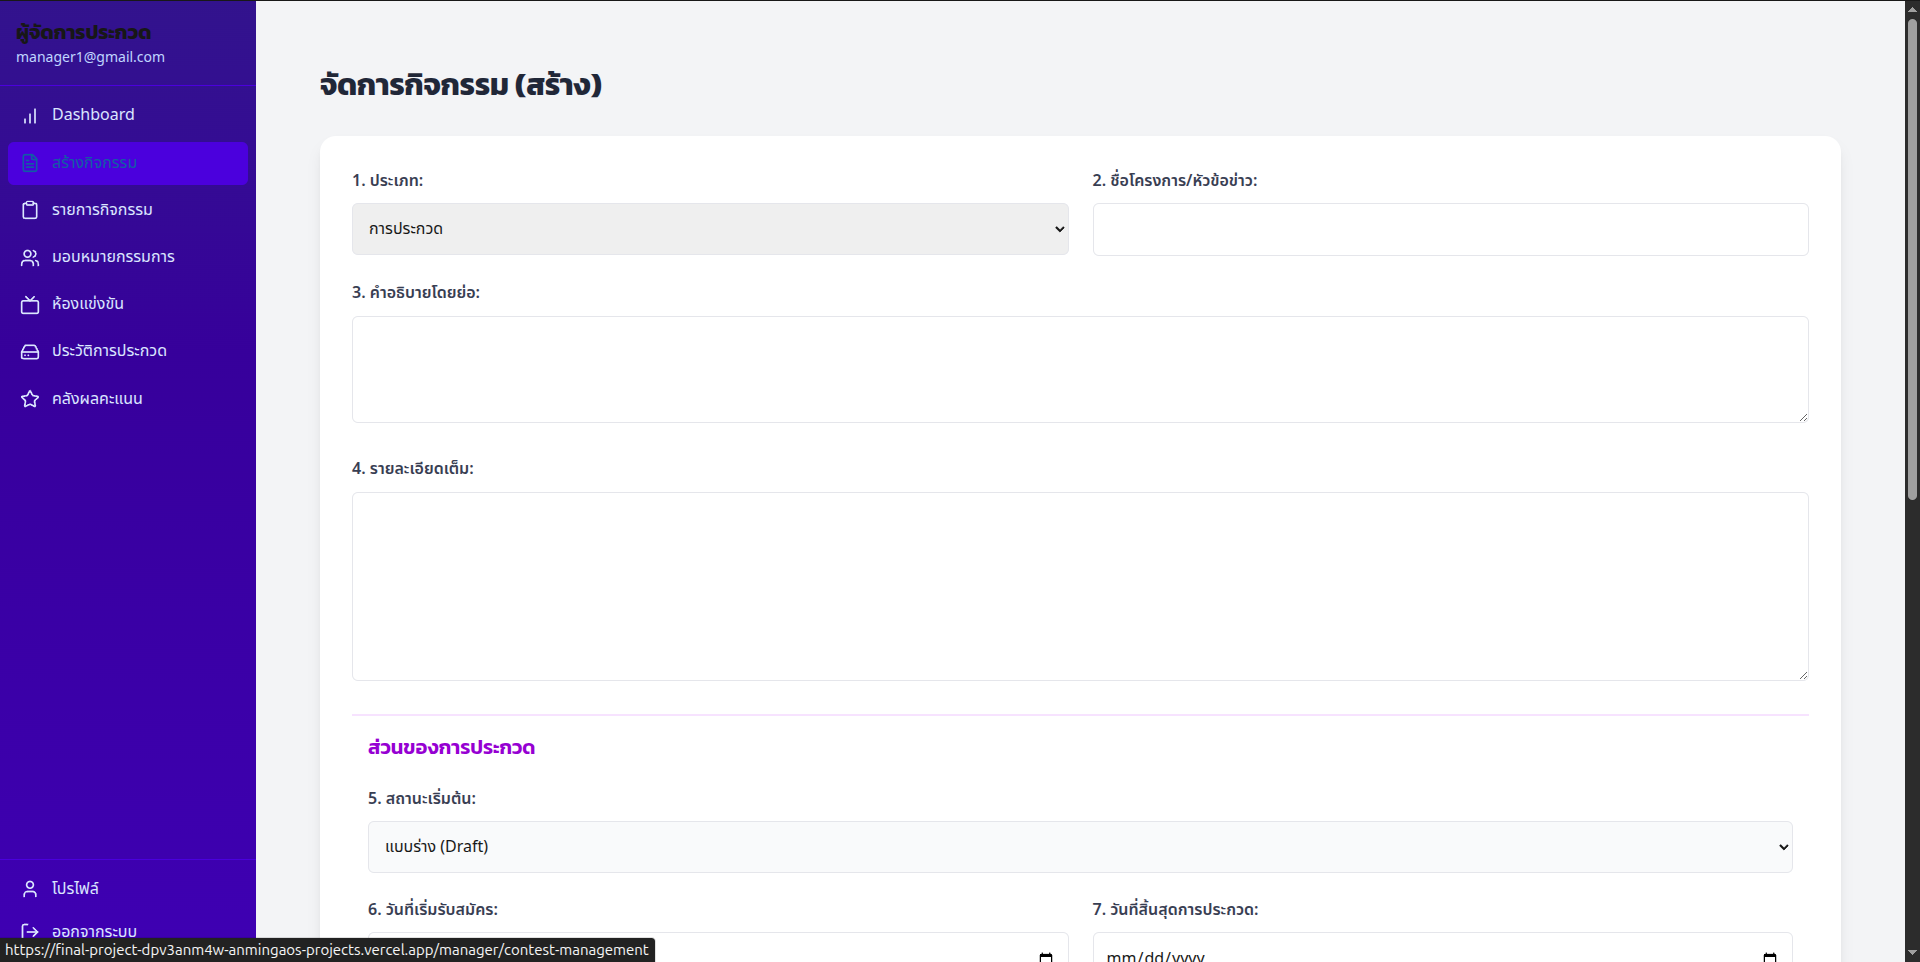
\includegraphics[width=0.8\linewidth]{MG2}
	\caption{หน้าสร้างกิจกรรมการประกวดหรือข่าวสาร}
\end{figure}

\indent หน้านี้เป็นหน้าที่ผู้จัดการใช้สำหรับ สร้าง "การประกวด" หรือ "ข่าวสาร" ใหม่ๆ เพื่อประกาศบนเว็บไซต์ โดยผู้จัดการจะต้องกรอกข้อมูลต่างๆ ให้ครบถ้วนตามแบบฟอร์ม

\newpage

\begin{figure}[h]
	\centering
	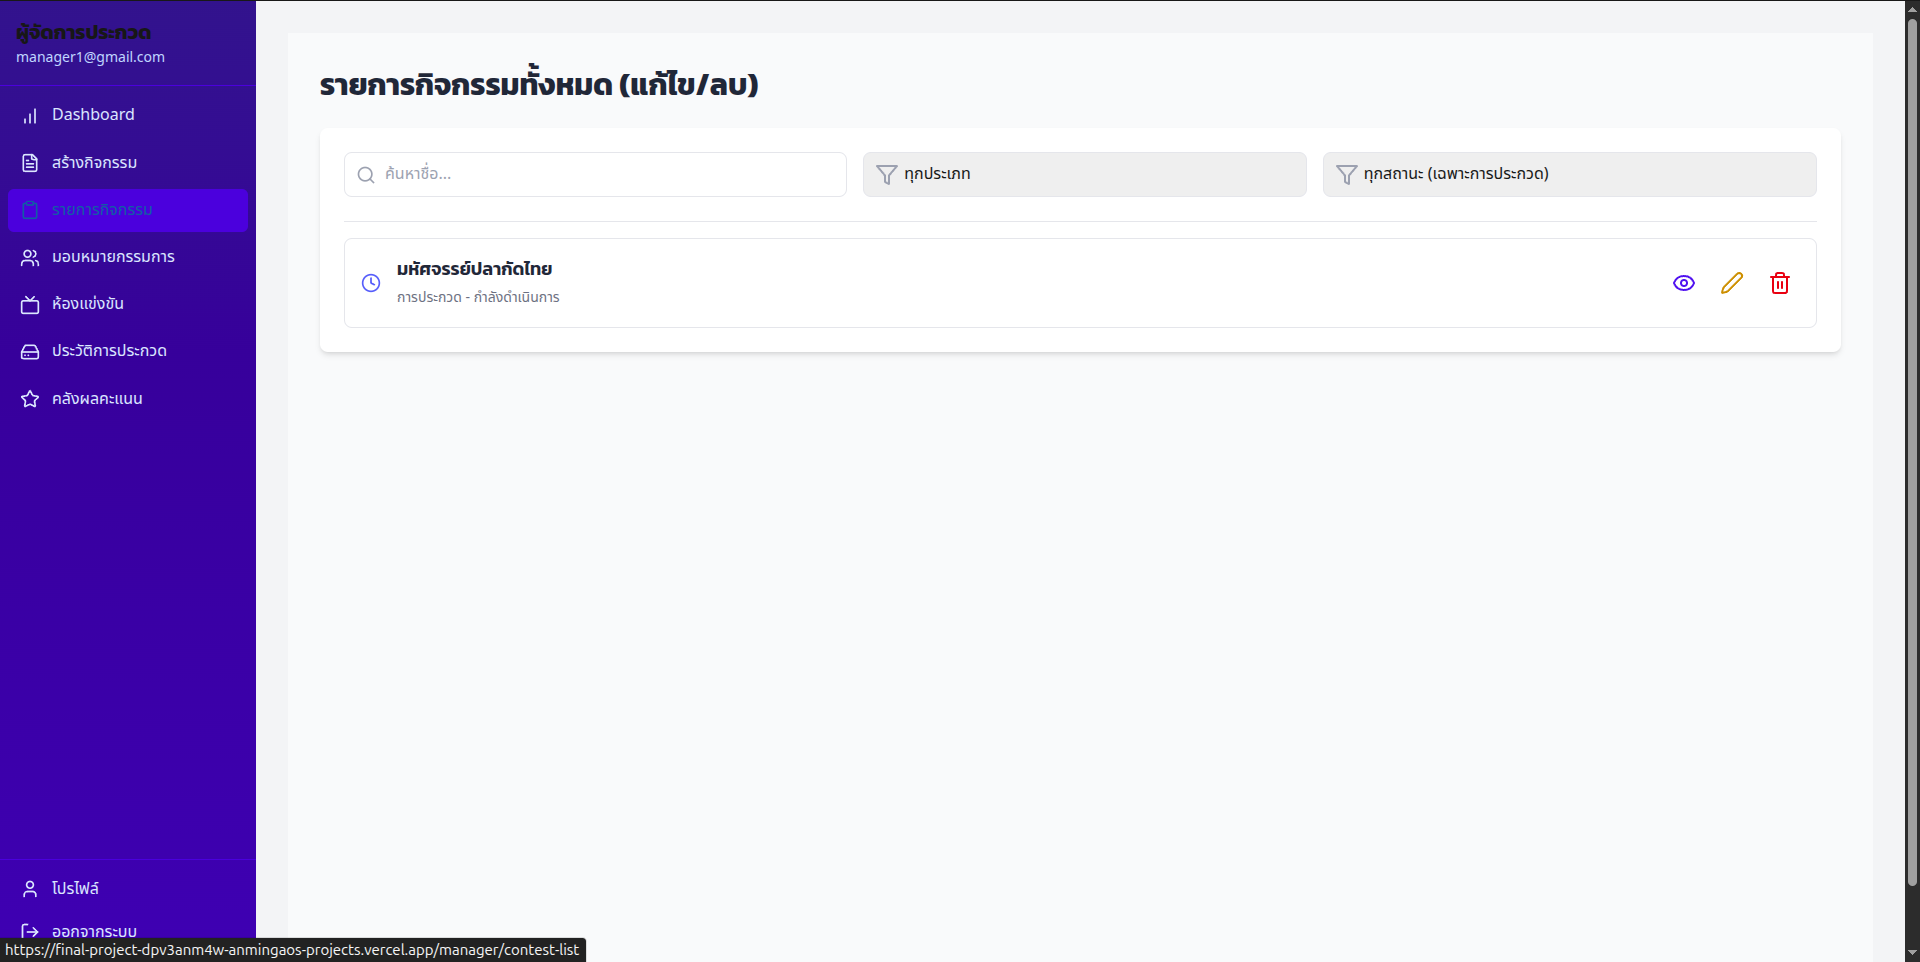
\includegraphics[width=0.8\linewidth]{MG3}
	\caption{หน้ากิจกรรมที่ได้สร้างขึ้นทั้งหมด}
\end{figure}

\indent หน้านี้เป็นเหมือนคลังเก็บกิจกรรมทั้งหมดที่ผู้จัดการเคยสร้างไว้ ไม่ว่าจะเป็น "การประกวด" หรือ "ข่าวสาร" ก็จะมารวมกันอยู่ที่นี่ทั้งหมด โดยผู้จัดการสามารถเข้ามาจัดการกิจกรรมต่างๆ ได้อย่างเต็มที่

\vspace{\baselineskip}

\begin{figure}[h]
	\centering
	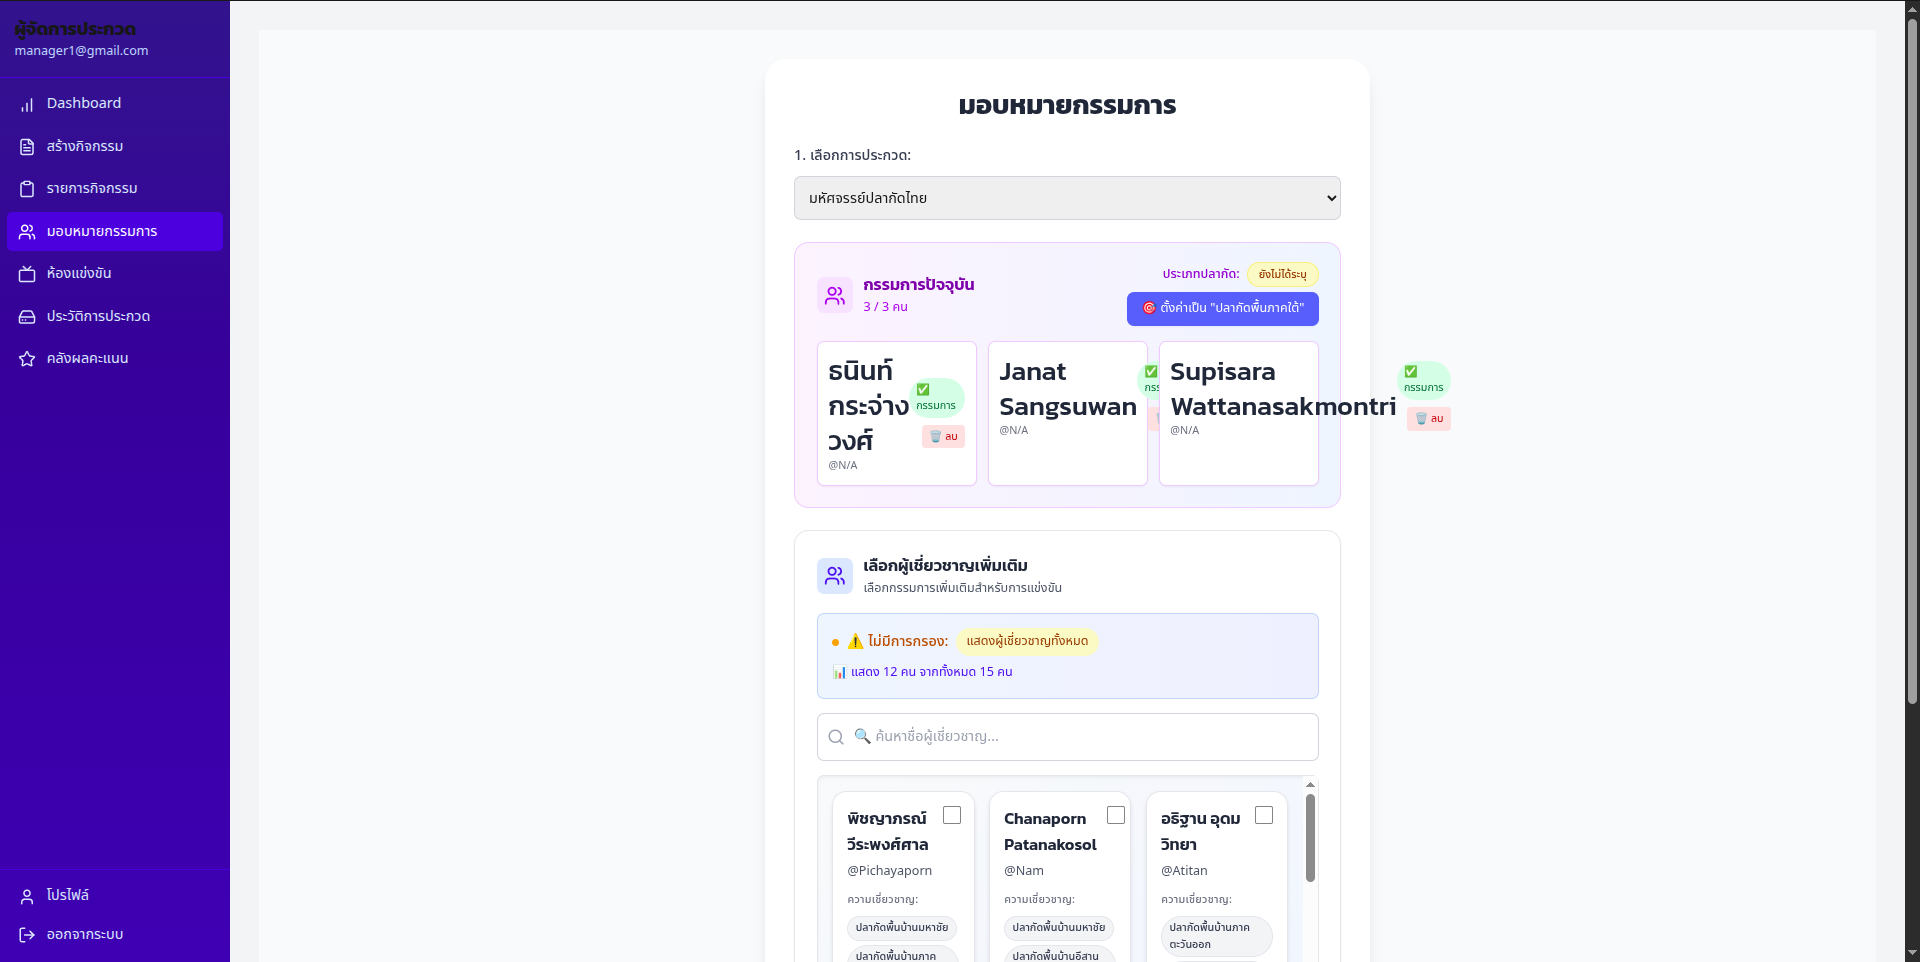
\includegraphics[width=0.8\linewidth]{MG4}
	\caption{หน้ามอบหมายกรรมการให้กิจกรรมการแข่งขัน}
\end{figure}

\indent นหน้านี้ ผู้จัดการสามารถเลือกการประกวด ผู้จัดการต้องใช้เมนู dropdown ด้านบนสุดเพื่อ เลือกการประกวด ที่ต้องการจะมอบหมายกรรมการก่อน ตรวจสอบกรรมการปัจจุบัน หลังจากเลือกการประกวดแล้ว ระบบจะแสดง "กรรมการปัจจุบัน" ที่ถูกมอบหมายให้งานนี้แล้วทำให้ผู้จัดการทราบว่าตอนนี้มีใครอยู่ในทีมตัดสินบ้าง

\newpage

\begin{figure}[h]
	\centering
	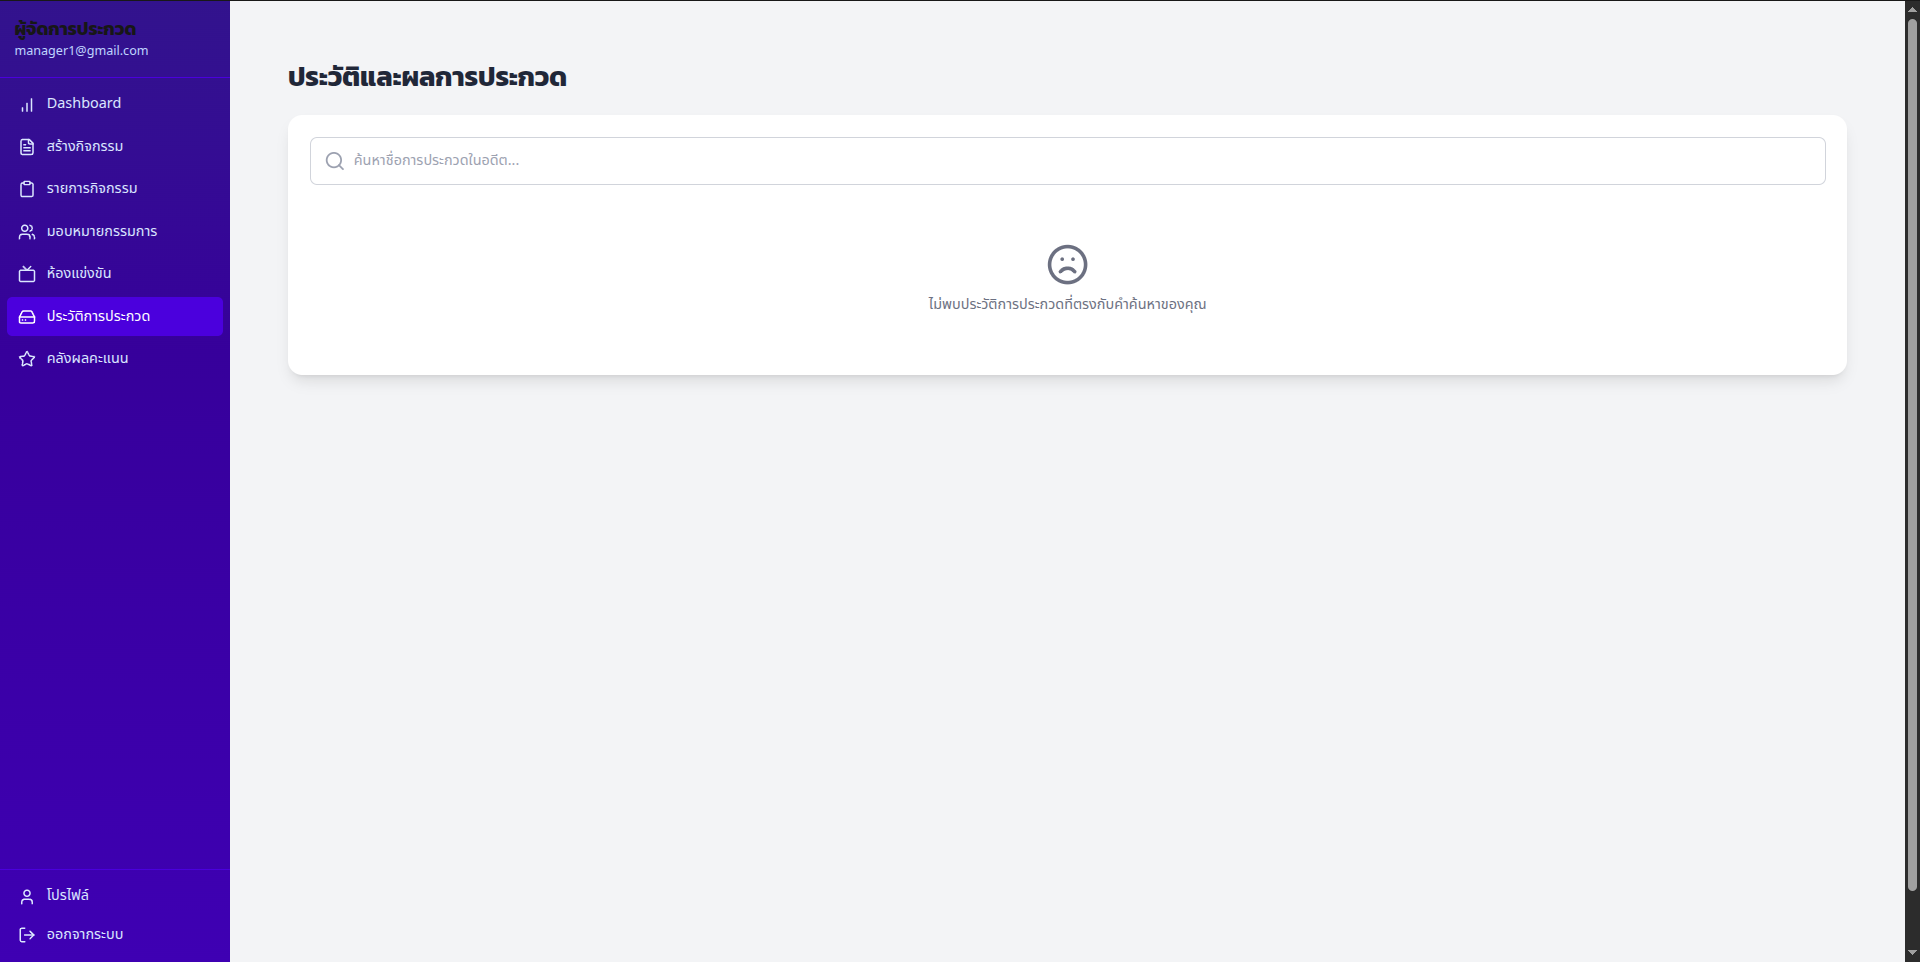
\includegraphics[width=0.8\linewidth]{MG6}
	\caption{หน้าประวติและผลการประกวด}
\end{figure}

\indent หน้านี้เปรียบเสมือนคลังเก็บข้อมูลสำหรับกิจกรรมการประกวดทั้งหมดที่ผู้จัดการเคยจัดและ เสร็จสิ้นไปแล้ว (เช่น ประกาศผลแล้ว หรือยกเลิกไป) ดูรายการประกวดที่จบไปแล้ว โดยปกติแล้ว หน้านี้จะแสดงรายการประกวดในอดีตทั้งหมดที่ผู้จัดการคนนี้เคยสร้างไว้ ทำให้สามารถย้อนกลับมาดูได้ว่าเคยจัดกิจกรรมอะไรไปบ้าง ดูผลสรุปการแข่งขัน คือส่วนที่สำคัญที่สุดครับ ในแต่ละรายการประกวดที่จบไปแล้ว จะมีปุ่ม "ดูผลสรุป" (ที่เป็นไอคอนรูปดวงตา) อยู่ข้างๆ เมื่อกดปุ่มนี้ จะมีหน้าต่าง Pop-up แสดงรายละเอียดผลการแข่งขันขึ้นมา ซึ่งจะบอกว่า ใครคือผู้ชนะ 3 อันดับแรก, ได้คะแนนรวมเท่าไหร่, และส่งปลาชื่ออะไรเข้าประกวด

\vspace{\baselineskip}

\begin{figure}[h]
	\centering
	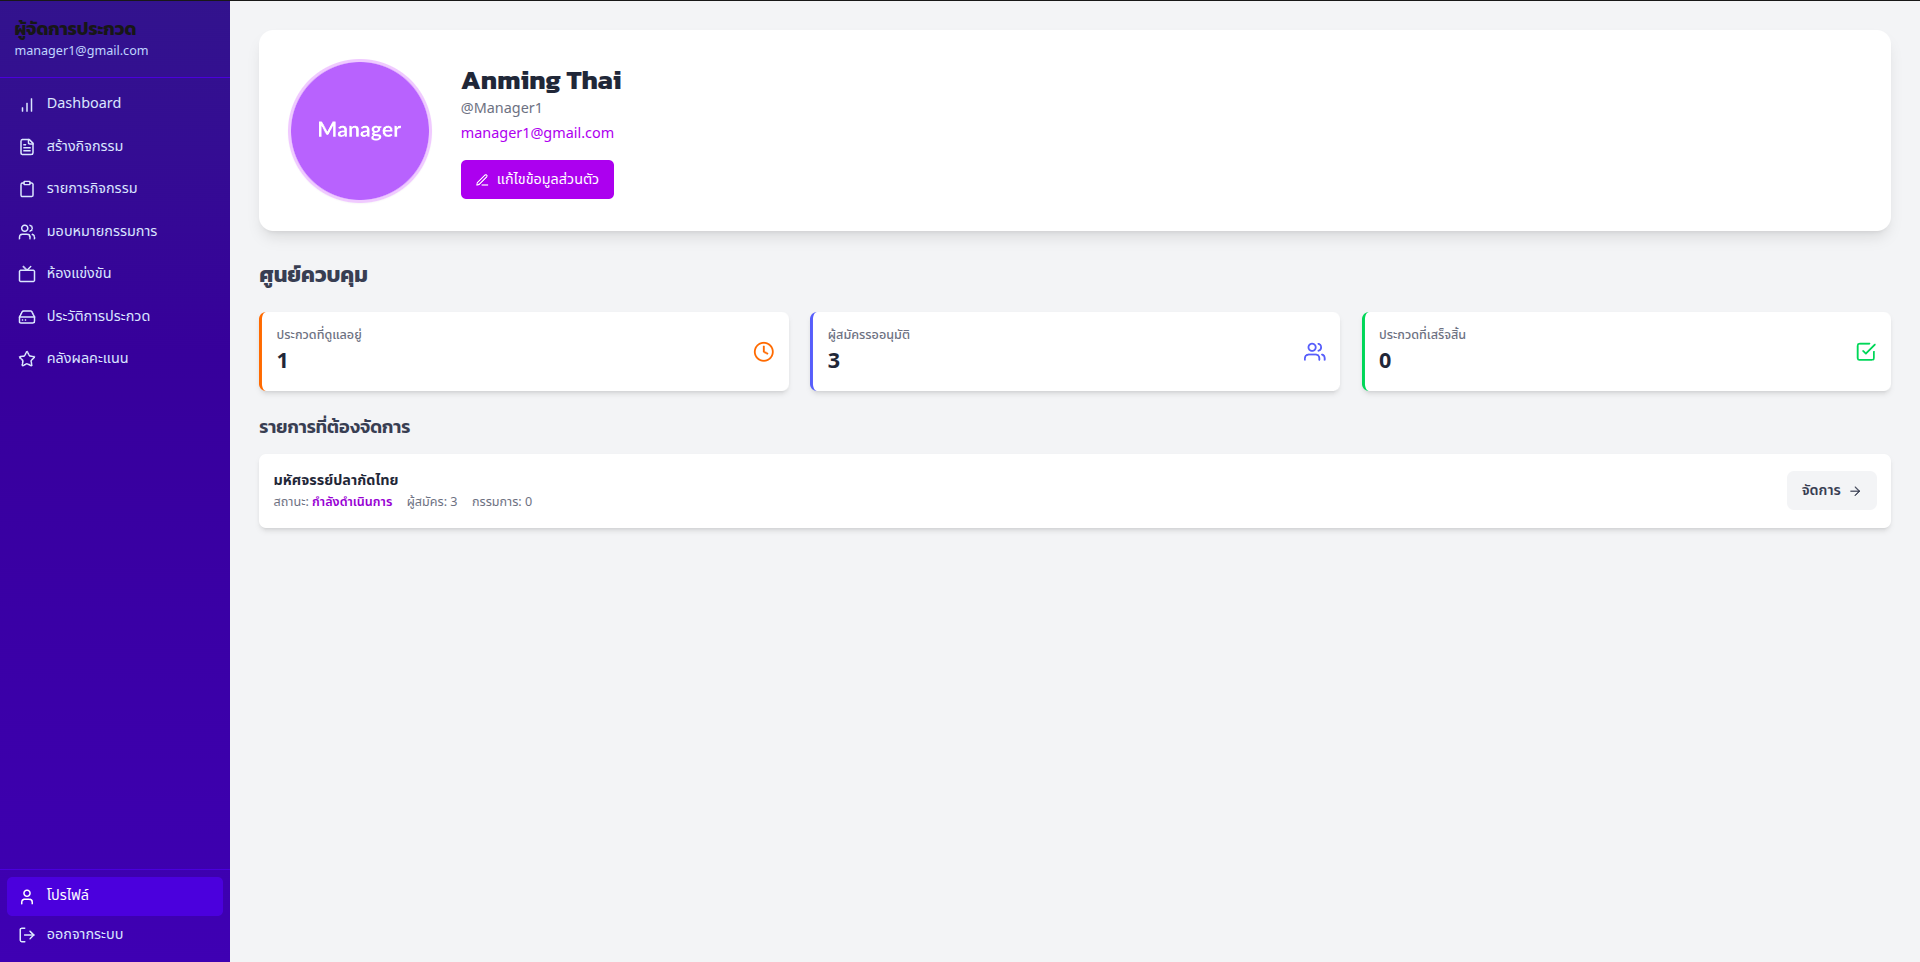
\includegraphics[width=0.8\linewidth]{MG8}
	\caption{หน้าโปรไฟล์ผู้จัดการประกวด}
\end{figure}

\indent ในหน้านี้ ผู้จัดการสามารถทำจัดการข้อมูลส่วนตัว จัดการจะเห็นข้อมูลของตัวเอง เช่น รูปโปรไฟล์, ชื่อ, และอีเมล สามารถกดปุ่ม "แก้ไขข้อมูลส่วนตัว" เพื่อเข้าไป เปลี่ยนชื่อ-นามสกุล หรือ Username ของตัวเองได้ สามารถ คลิกที่รูปโปรไฟล์ เพื่ออัปโหลดรูปประจำตัวใหม่ได้ และยังสามารถภาพรวมและจัดการงานด่วน  ศูนย์ควบคุม จะมีสรุปตัวเลขสำคัญๆ ให้ดูอย่างรวดเร็ว เช่น ตอนนี้มี "ประกวดที่ดูแลอยู่" กี่รายการ, มี "ผู้สมัครรออนุมัติ" กี่คน, และมี "ประกวดที่เสร็จสิ้น" ไปแล้วกี่รายการ รายการที่ต้องจัดการ ส่วนนี้สำคัญมากจะแสดงรายการประกวดที่กำลังดำเนินการอยู่ (Active) ผู้จัดการสามารถดูสถานะคร่าวๆ และกดปุ่ม "จัดการ" ที่ท้ายรายการได้เลย เมื่อกดปุ่ม "จัดการ" ระบบจะพาผู้จัดการเข้าไปที่ "ห้องแข่งขัน" (Live Contest Room) ของการประกวดนั้นๆ ทันที เพื่อไปอนุมัติผู้สมัครหรือจัดการขั้นตอนต่อไป

\endgroup